%%-----------------------------------------------------------------------------
%%                           DOCUMENT INFO
%%
%%-----------------------------------------------------------------------------
\documentclass[12pt,compress,handout]{beamer}  %For printable version
%\documentclass[12pt,compress]{beamer}         %For presentation version

%% -------------- Packages ------------------------------
\usepackage{amssymb}
\usepackage{amsmath}
\usepackage{amsthm}
\usepackage{colortbl}
\usepackage{graphicx}
\usepackage{hyperref}
\usepackage[sort]{natbib}
\usepackage{rotating}
\usepackage{subfigure}
\usepackage{multirow}
\usepackage{tikz}
\usetikzlibrary{shapes,arrows,trees,snakes,positioning,fit,shadows}     % library for tikz
\usepackage{bm}
\usepackage{epstopdf}
\usepackage{setspace}
\usepackage{bigstrut}
\usepackage{caption}
\usepackage{longtable}
\usepackage{lscape}
\usepackage{epstopdf}
\usepackage{multirow}
\usepackage{enumerate}
\usepackage{csquotes}
\usepackage{pdfpages}
\usepackage{float}
\usepackage{booktabs}

%% ----- Theme and formatting for printable version ---------
\mode<handout>{
  \useoutertheme{split}
  \useinnertheme{rounded}
  \usecolortheme{seahorse}
  \usecolortheme{rose}
  %\setbeamertemplate{footline}[frame number]
  \usepackage{pgfpages}
  %\pgfpagesuselayout{resize to}[letterpaper,landscape]

  \setbeamertemplate{footline}
{
 \leavevmode%
 \hbox{%
 \begin{beamercolorbox}[wd=.3\paperwidth,ht=2.25ex,dp=1ex,center]{author in head/foot}%
   \usebeamerfont{author in head/foot}\insertshortauthor~~%\beamer@ifempty{\insertshortinstitute}{}{(\insertshortinstitute)
 \end{beamercolorbox}%
 \begin{beamercolorbox}[wd=.6\paperwidth,ht=2.25ex,dp=1ex,center]{title in head/foot}%
   \usebeamerfont{title in head/foot}\insertshorttitle
 \end{beamercolorbox}%
 \begin{beamercolorbox}[wd=.1\paperwidth,ht=2.25ex,dp=1ex,right]{date in head/foot}%
   %\usebeamerfont{date in head/foot}\insertshortdate{}\hspace*{2em}
   \insertframenumber{} / \inserttotalframenumber\hspace*{2ex}
 \end{beamercolorbox}}%
 \vskip0pt%
}
}

%% ----- Theme for projector DYNAMIC display version --------------
\mode<beamer>{
  \useoutertheme{shadow}
  \usecolortheme{whale}
  \usecolortheme{orchid}
  \useinnertheme[shadow=true]{rounded}
  \setbeamerfont{block title}{size={}}
  \hypersetup{pdfpagemode=FullScreen}

  \setbeamertemplate{footline}
{
 \leavevmode%
 \hbox{%
 \begin{beamercolorbox}[wd=.5\paperwidth,ht=2.25ex,dp=1ex,center]{author in head/foot}%
   \usebeamerfont{author in head/foot}\insertshortauthor~~%\beamer@ifempty{\insertshortinstitute}{}{(\insertshortinstitute)
 \end{beamercolorbox}%
 \begin{beamercolorbox}[wd=.5\paperwidth,ht=2.25ex,dp=1ex,center]{title in head/foot}%
   \usebeamerfont{title in head/foot}\insertshorttitle
 \end{beamercolorbox}%
 }%
 \vskip0pt%
}
}

%% ----- Formatting for beamer ----------------------------
\mode<handout>{
\setbeamertemplate{headline}
{
  \leavevmode%
  \hbox{%
    \begin{beamercolorbox}[wd=\paperwidth,ht=2.25ex,dp=1ex,center]{section in head/foot}%
      \insertsectionnavigationhorizontal{\paperwidth}{}{}%
     \end{beamercolorbox}}
  \vskip0pt%
}
}

\mode<beamer>{
\setbeamertemplate{headline}
{
  \leavevmode%
  \hbox{%
    \begin{beamercolorbox}[wd=\paperwidth,ht=2.25ex,dp=1ex,center]{section in head/foot}%
      \insertsectionnavigationhorizontal{\paperwidth}{}{}%
     \end{beamercolorbox}}
  \vskip2pt%
}
}

\setbeamertemplate{mini frames}[default]%
\setbeamertemplate{sections/subsections in toc}[ball]%
\setbeamertemplate{mini frame in other subsection}[default][0]%
\setbeamertemplate{frametitle continuation}[from second]%
\setbeamersize{text margin left=0.2 in}%
\setbeamersize{text margin right=0.2 in}%
\setbeamerfont{frametitle}{size=\small}%
\setbeamerfont{infolines}{size=\footnotesize}%

%% ----- The next 3 lines allow natbib to work properly in a Beamer Document --
\makeatletter
\def\newblock{\beamer@[EMAIL PROTECTED]}
\makeatother

%%----- User-defined LaTeX commands (cruft from numerous older versions) ------

\newcommand{\orth}{\ensuremath{\perp\!\!\!\perp}}%

\DeclareMathAlphabet{\mathitbf}{OML}{cmm}{b}{it}

\renewcommand{\figurename}{Figure~\arabic{figure}}
\renewcommand{\tablename}{Table~\arabic{table}}

%\newcounter{thmcnt}
%\newtheorem{thm}{Theorem \arabic{thmcnt}}
%
%
%%%%%%%%%%%%%%%%%%%%%%%%%%%%%%%%%%%%%%%%%%%%%%%%%%%%%%%%%%%%%%%%%%%%%%%%%%%%%%%
%% User-defined LaTeX commands
%\DeclareMathOperator*{\Cov}{Cov} \DeclareMathOperator*{\Var}{Var}
%\DeclareMathOperator*{\argmax}{argmax}
%\newcommand{\notorth}{\ensuremath{\perp\!\!\!\!\!\!\diagup\!\!\!\!\!\!\perp}}
%\newcommand{\orthog}{\ensuremath{\perp\!\!\!\perp}}
%\newcommand{\orth}{\ensuremath{\perp\!\!\!\perp}}


%%%%%%%%%%%%%%%%%%%%%%%%%%%%%%%%%%%%%%%%%%%%%%%%%%%%%%%%%%%%%%%%%%%%%%%%%%%%%%
\begin{document}


%%%%%%%%%%%%%%%%%%%%%%%%%%%%%%%%%%%%%%%%%%%%%%%%%%%%%%%%%%%%%%%%%%%%%%%%%%%%%%%
\title{Generalized Ben-Porath Model}

\author{James Heckman}

\date{Econ 350 \\
This draft, \today}


%%%%%%%%%%%%%%%%%%%%%%%%%%%%%%%%%%%%%%%%%%%%%%%%%%%%%%%%%%%%%%%%%%%%%%%%%%%%%%%
\frame{\titlepage}


%%%%%%%%%%%%%%%%%%%%%%%%%%%%%%%%%%%%%%%%%%%%%%%%%%%%%%%%%%%%%%%%%%%%%%%%%%%%%%
\begin{frame}[plain]
\frametitle{Table 1. Estimates of the human capital production
function (males)$^{\text{a}}$.}
\begin{center}
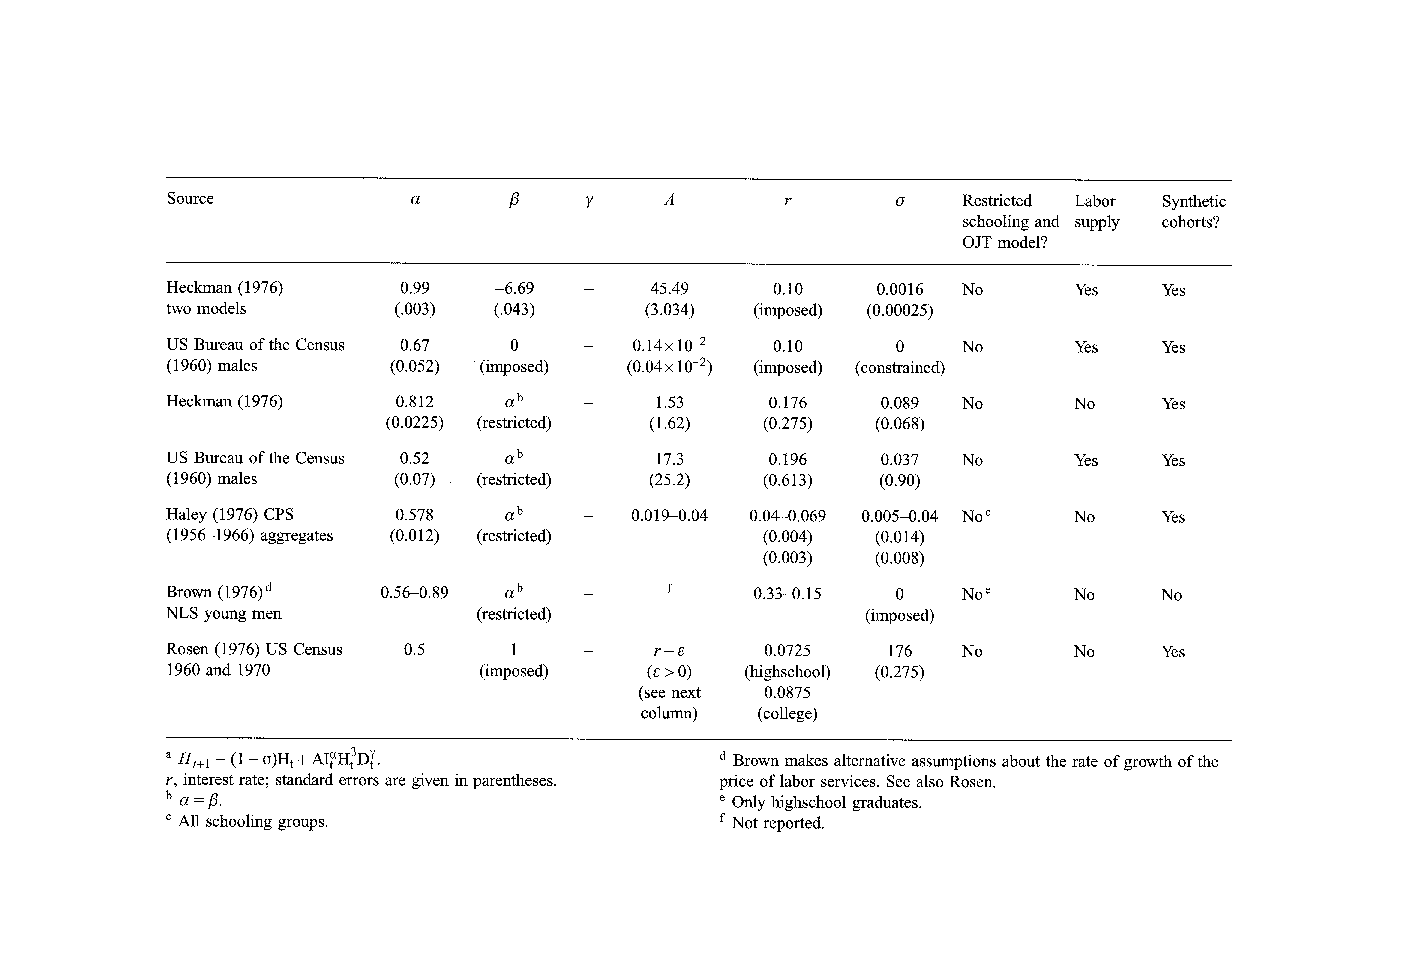
\includegraphics[width=4.5in]{include/tab-bbh-est-hum-cap.pdf}

{\footnotesize Source: Browning, Hansen and Heckman (1999)}
\end{center}
\end{frame}


%%%%%%%%%%%%%%%%%%%%%%%%%%%%%%%%%%%%%%%%%%%%%%%%%%%%%%%%%%%%%%%%%%%%%%%%%%%%%%%
\begin{frame}
\frametitle{Table 2 (references cited)}
\begin{itemize}[<+->]
\item Heckman, J.J. (1976), ``A life-cycle model of earnings, learning, and consumption'', \emph{Journal of Political
Economy} 84(4, pt. 2): S11--S44.

\item US Bureau of the Census (1960), 1960 Census Public Use Sample (United States Government Printing
Office, Washington, DC).

\item Haley, W.J. (1976), ``Estimation of the earnings profile from optimal human capital accumulation'',
\emph{Econometrica} 44: 1223--38.

\item Brown, C. (1976), ``A model of optimal human-capital accumulation and the wages of young high school
graduates'', \emph{Journal of Political Economy} 84(2): 299--316.

\item Rosen, S. (1976), ``A theory of life earnings'', \emph{Journal of Political Economy} 84(Suppl.): 345--382.
\end{itemize}
\end{frame}


%%%%%%%%%%%%%%%%%%%%%%%%%%%%%%%%%%%%%%%%%%%%%%%%%%%%%%%%%%%%%%%%%%%%%%%%%%%%%%
\begin{frame}[plain]
\frametitle{Table 2. Estimated parameters for human capital
production function.}
\begin{center}
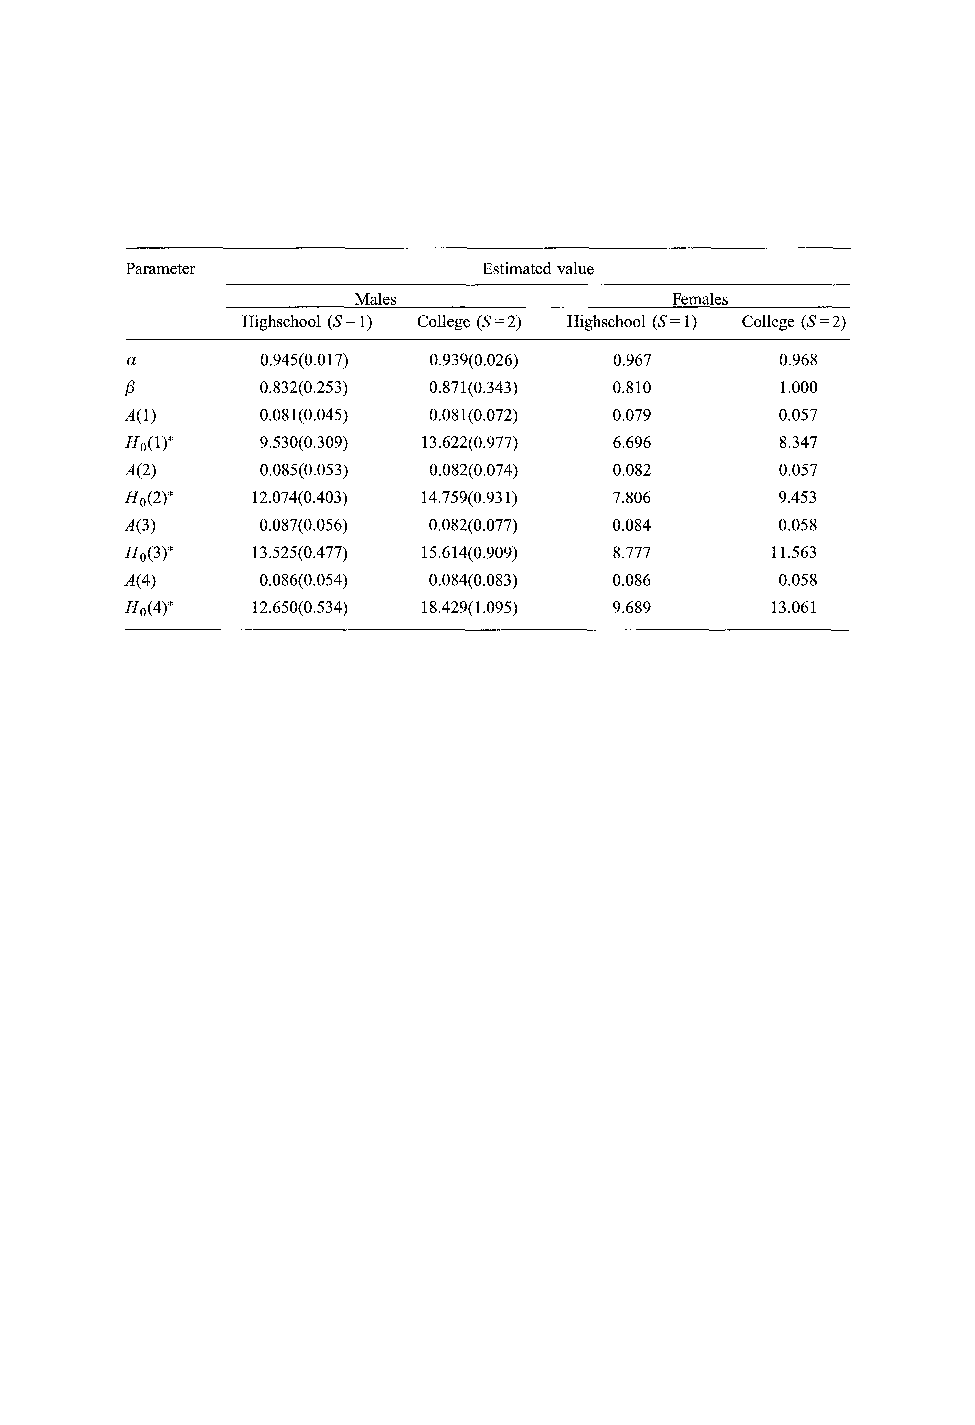
\includegraphics[width=4.5in]{include/tab-bbh-est-param-hum-cap.pdf}

{\footnotesize Source: Heckman, Lochner and Taber (1998)}
\end{center}
\end{frame}


%%%%%%%%%%%%%%%%%%%%%%%%%%%%%%%%%%%%%%%%%%%%%%%%%%%%%%%%%%%%%%%%%%%%%%%%%%%%%%%
\begin{frame}
\frametitle{Table 2 (notes)}
\begin{itemize}[<+->]
\item Human capital production function: $H_{a+1}^{S} = A^{S}(\theta)
(I_{a}^{S})^{\alpha_{S}} (H_{a}^{S})^{\beta_{S}} + (1 -\sigma)
(H_{a}^{S})^{\beta_{S}}$, with $S=1,2$. Standard errors are given in
parentheses.

\item Heckman, Lochner and Taber (1999) do not report the standard
errors for females.

\item Initial human capital for person of ability quantile using
ability levels for NLSY.
\end{itemize}
\end{frame}


%%%%%%%%%%%%%%%%%%%%%%%%%%%%%%%%%%%%%%%%%%%%%%%%%%%%%%%%%%%%%%%%%%%%%%%%%%%%%%%
\begin{frame}
\begin{itemize}[<+->]
\item
Convention: $H(t),I(t)$ written as $I,H$ unless it clarifies matters not doing so.
\item
Consider a more general Ben-Porath Model
\begin{equation*}
\dot{H}=AI^{\alpha }H^{\beta }-\sigma H
\end{equation*}
Neutrality: $\alpha =\beta$.

\item
For simplicity assume no discounting $(r=0)$

\item
No depreciation $\sigma =0$

\item
Finite life $=T$

\item
Rental rate $=R$ (efficiency units, price of human capital)

\item
Initial endowment $=H_{0}$
\end{itemize}
\end{frame}


%%%%%%%%%%%%%%%%%%%%%%%%%%%%%%%%%%%%%%%%%%%%%%%%%%%%%%%%%%%%%%%%%%%%%%%%%%%%%%%
\begin{frame}
\begin{itemize}[<+->]
\item Problem ($0\leq I\leq 1$; $0<\alpha <1$ for smooth problems):
\begin{equation*}
\max \int_{0}^{T}[RH(t)-RI(t)H(t)]dt
\end{equation*}
such that $\dot{H} =AI^\alpha H^{\beta }$ and $H(0)=H_0$.

\item
Hamiltonian for problem:\\
Maximized Hamilton must be concave in state variable:
\begin{equation*}
\mathcal{H}=RH(t)(1-I(t))+\mu (AI^\alpha H^\beta )
\end{equation*}
$\beta \leq 1$ needed for Mangasarian sufficient conditions.
\end{itemize}
\end{frame}


%%%%%%%%%%%%%%%%%%%%%%%%%%%%%%%%%%%%%%%%%%%%%%%%%%%%%%%%%%%%%%%%%%%%%%%%%%%%%%%
\begin{frame}
\begin{itemize}[<+->]
\item
FOC:
\begin{equation}
\mu A\alpha I^{\alpha -1}H^\beta \geq RH \tag{$*$} \label{eq:old-doritos}
\end{equation}

\item
Let ``\,$\dot{~}$\,'' denote time rate of change.
\begin{equation*}
\dot{\mu} =-\frac{\partial \mathcal{H}}{\partial H} =-R(1-I)-\beta
\mu AI^\alpha H^{\beta -1}
\end{equation*}

\item
Rate of change of the shadow value of human capital declines with
increases in the human capital stock.

\item
$\mu (T)H(T) = 0$ (transversality)
\begin{equation*}
\mu(t) = \int_{t}^{T} \left[ R(1 - I(u)) + \beta (\mu(u)) AI^{\alpha
- 1}(u) H^{\beta - 1} (u) \right]\,du
\end{equation*}
\end{itemize}
\end{frame}


%%%%%%%%%%%%%%%%%%%%%%%%%%%%%%%%%%%%%%%%%%%%%%%%%%%%%%%%%%%%%%%%%%%%%%%%%%%%%%%
\begin{frame}
\begin{itemize}[<+->]
\item
Now for the case with strict inequality in (\ref{eq:old-doritos}),
we have $I=1$ (period of specialization  associated with schooling
or no earnings).
\begin{align*}
\alpha \mu AH^\beta >& RH \\
H^{\beta -1} >& \frac R{\alpha \mu A}
\end{align*}

\item
If $\beta >1$, we get specialization in investment (no work) if
\begin{equation*}
H>\left[ \frac R{\alpha \mu A}\right] ^{\frac 1{\beta -1}}.
\end{equation*}
\end{itemize}
\end{frame}


%%%%%%%%%%%%%%%%%%%%%%%%%%%%%%%%%%%%%%%%%%%%%%%%%%%%%%%%%%%%%%%%%%%%%%%%%%%%%%%
\begin{frame}
\begin{itemize}[<+->]
\item
Specialization at $t=0$ requires
\begin{equation*}
H_0>\left[ \frac R{\alpha \mu (0)A}\right] ^{\frac 1{\beta
-1}}=\left( \frac R{\alpha A}\right) ^{\frac 1{\beta -1}}(\mu_{0}
)^{\frac 1{1-\beta }}
\end{equation*}
\end{itemize}
\end{frame}


%%%%%%%%%%%%%%%%%%%%%%%%%%%%%%%%%%%%%%%%%%%%%%%%%%%%%%%%%%%%%%%%%%%%%%%%%%%%%%%
\begin{frame}
\begin{itemize}[<+->]
\item
If $\beta <1$, specialization at $t=0$ requires
\begin{equation*}
H_0<\left[ \frac R{\alpha \mu (0)A}\right] ^{\frac 1{\beta
-1}}=\left( \frac R{\alpha A}\right) ^{\frac 1{\beta -1}}\left( \mu
_0\right) ^{\frac 1{1-\beta }}.
\end{equation*}

\item
When $\beta =1$, specialization at $t=0$ requires $\mu_{0} >\dfrac
R{\alpha A}$.
\end{itemize}
\end{frame}


%%%%%%%%%%%%%%%%%%%%%%%%%%%%%%%%%%%%%%%%%%%%%%%%%%%%%%%%%%%%%%%%%%%%%%%%%%%%%%%
\begin{frame}
\begin{itemize}[<+->]
\item
Person just specializing ($I=1$ is the interior solution) if
\begin{align*}
\alpha \mu AH^\beta &=RH \qquad \qquad (I=1) \\
\mu &=\left( \frac R{\alpha A}\right) H^{1-\beta }
\end{align*}

\item
In a period of specialization, $I=1$
\begin{align*}
\dot{\mu} &= -\beta \mu AH^{\beta -1} \\
\dot{H} &= AH^\beta
\end{align*}

\item
Then,
\begin{equation*}
\frac{\dot{H}}{H^{\beta }} =A \qquad \text{or} \qquad
\frac{dH}{H^{\beta }} = Adt
\end{equation*}
\end{itemize}
\end{frame}


%%%%%%%%%%%%%%%%%%%%%%%%%%%%%%%%%%%%%%%%%%%%%%%%%%%%%%%%%%%%%%%%%%%%%%%%%%%%%%%
\begin{frame}
\begin{gather*}
\frac{[H(t)]^{1-\beta }}{1-\beta } =At+c_{0}\quad ,\quad \beta \neq 1 \\
\\
H(t) =(At+c_{0})^{\frac{1}{1-\beta }}(1-\beta )^{\frac{1}{1-\beta }}
\end{gather*}
(making $t$ dependence explicit)

\begin{gather*}
H(0) =H_{0}=c_{0}^{\frac{1}{1-\beta }}(1-\beta )^{\frac{1}{1-\beta }} \\
\\
\left( \frac{H_{0}}{(1-\beta )^{\frac{1}{1-\beta }}}\right)
^{1-\beta } =c(0).
\end{gather*}
\end{frame}


%%%%%%%%%%%%%%%%%%%%%%%%%%%%%%%%%%%%%%%%%%%%%%%%%%%%%%%%%%%%%%%%%%%%%%%%%%%%%%%
\begin{frame}
\begin{itemize}[<+->]
\item
When $\beta =1$,
\begin{align*}
\ln H(t) &= At+c_{0} \\
H(t) &= e^{At+c_{0}} \\
H(0) &= H_{0}=e^{c_{0}}\qquad \qquad \ln H_{0}=c_{0}.
\end{align*}
\end{itemize}
\end{frame}


%%%%%%%%%%%%%%%%%%%%%%%%%%%%%%%%%%%%%%%%%%%%%%%%%%%%%%%%%%%%%%%%%%%%%%%%%%%%%%%
\begin{frame}
\begin{itemize}[<+->]
\item
When $\beta \neq 1$,
\begin{gather*}
\dot{\mu} = -\beta \mu A[H]^{\beta -1} = -\beta \mu A\left[ \frac{1}{(At+c_{0})(1-\beta )}\right] \\
\\
\frac{\dot{\mu}}{\mu }=\frac{-\beta }{1-\beta }\cdot \frac{A}{At+c_{0}}\qquad \qquad c_{0}\geq 0 \\
\\
\ln \mu (t) = -\left( \frac{\beta }{1-\beta }\right) \cdot \ln
(At+c_{0}) +c_{1} \\
\\
\mu (t) = e^{c_{1}}e^{-\frac{\beta }{1-\beta }\ln (At+c_{0})} =
\frac{e^{c_{1}}}{(At+c_{0})^{\beta /1-\beta }}
\end{gather*}
\end{itemize}
\end{frame}


%%%%%%%%%%%%%%%%%%%%%%%%%%%%%%%%%%%%%%%%%%%%%%%%%%%%%%%%%%%%%%%%%%%%%%%%%%%%%%%
\begin{frame}
\begin{itemize}[<+->]
\item
At $t=0$,
\begin{gather*}
\mu (0)=\frac{e^{c_{1}}}{c_{0}^{\beta /1-\beta }} =
\frac{e^{c_{1}}}{\left( \frac{H(0)}{(1-\beta )^{\frac{1}{1-\beta
}}}\right) } = \frac{e^{c_{1}}}{H(0)^{\beta }}(1-\beta )^{\beta
/1-\beta } \\
\\
\frac{\mu (0)H(0)^{\beta }}{(1-\beta )^{\beta /1-\beta }} = e^{c_{1}} \\
\\
c_{1} = \ln \left[ \frac{\mu (0)[H(0)]^{\beta }}{(1-\beta )^{\beta
/1-\beta }}\right] .
\end{gather*}
\end{itemize}
\end{frame}


%%%%%%%%%%%%%%%%%%%%%%%%%%%%%%%%%%%%%%%%%%%%%%%%%%%%%%%%%%%%%%%%%%%%%%%%%%%%%%%
\begin{frame}
\begin{itemize}[<+->]
\item
When $\beta =1$,
\begin{gather*}
\frac{\dot{\mu}}{\mu } =-A \\
\\
\ln \mu (t) = -At+c_{1}^{*} \\
\\
\mu (t) = e^{c_{1}^{*}}e^{-At} \\
\\
\mu (0) = e^{c_{1}^{*}}\qquad \ln \mu (0)=c_{1}^{*}
\end{gather*}
\end{itemize}
\end{frame}


%%%%%%%%%%%%%%%%%%%%%%%%%%%%%%%%%%%%%%%%%%%%%%%%%%%%%%%%%%%%%%%%%%%%%%%%%%%%%%%
\begin{frame}
\begin{itemize}[<+->]
\item
Now at end of period of specialization, we must have
\begin{equation*}
\mu (t^{*})A\alpha [H(t)]^{\beta }=RH(t).
\end{equation*}

\item
Thus for $\beta =1$, specialization ends (schooling ends) when
\begin{gather*}
\mu (t^{*})A\alpha = R \qquad \qquad \mu (t^{*}) = \left( \frac{R}{A\alpha }\right) \\
\\
e^{c_{1}^{*}}e^{-At^{*}} = \left( \frac{R}{A\alpha }\right) \qquad \qquad \frac{e^{c_{1}^{*}}A\alpha }{R} = e^{At^{*}} \\
\\
c_{1}^{*}+\ln \left( \frac{A\alpha }{R}\right) = At^{*} \qquad
\qquad \frac{1}{A}\left[ c_{1}^{*}+\ln \left( \frac{A\alpha
}{R}\right) \right] = t^{*}.
\end{gather*}
\end{itemize}
\end{frame}


%%%%%%%%%%%%%%%%%%%%%%%%%%%%%%%%%%%%%%%%%%%%%%%%%%%%%%%%%%%%%%%%%%%%%%%%%%%%%%%
\begin{frame}
\begin{itemize}[<+->]
\item
When $\beta \neq 1$
\begin{equation*}
\mu (t^{*})\frac{A\alpha }{R} = [H(t^{*})]^{1-\beta } \qquad
H(t^{*}) = \left[ \frac{\mu (t^{*})A\alpha }{R}\right]
^{\frac{1}{1-\beta }}.
\end{equation*}

\item
Substituting from above we find that we get
\begin{equation*}
\frac{e^{c_{1}}}{(At+c_{0})^{\beta /1-\beta }}\frac{A\alpha
}{R}=(At+c_{0})(1-\beta ).
\end{equation*}
\end{itemize}
\end{frame}


%%%%%%%%%%%%%%%%%%%%%%%%%%%%%%%%%%%%%%%%%%%%%%%%%%%%%%%%%%%%%%%%%%%%%%%%%%%%%%%
\begin{frame}
\begin{itemize}[<+->]

\item
The Ben Porath case is $\alpha =\beta $.

\item
Therefore, $\dot{\mu} =-R$ (trivial dynamics).
\begin{align*}
\mu (t) &= -Rt+c_{1},\quad \mu (T)=0 \Rightarrow c_{1}=RT \\
\mu (t) &= -R(T-t)
\end{align*}

\item
General case:
\begin{align*}
\dot{\mu} &= R\left[ -1+\underset{I}{\underbrace{R^{\frac{1}{\alpha
-1}}\left( \frac{1}{A}\right) ^{\frac{1}{1-\alpha }}\alpha
^{\frac{1}{1-\alpha }}\mu ^{\frac{1}{1-\alpha }}H^{\frac{\beta
-1}{1-\alpha }}}}\left(
1-\beta /\alpha \right) \right] \\
\\
&= R[-1+I\,\,\,\underset{\text{adjustment to
}I}{\underbrace{(1-\beta /\alpha )}}]
\end{align*}
\end{itemize}
\end{frame}


%%%%%%%%%%%%%%%%%%%%%%%%%%%%%%%%%%%%%%%%%%%%%%%%%%%%%%%%%%%%%%%%%%%%%%%%%%%%%%%
\begin{frame}
\begin{itemize}[<+->]
\item
Therefore, we have that if $\beta /\alpha >1$, $\dot{\mu} < 0$.
\medskip
\item
If $\beta < 0$, $\dot{\mu}$ might be $>0$.
\medskip
\item
Assume for the moment that $\beta \geq 0$. Then what do we have?
\medskip
\item
$\dot{\mu} =-R$ during period of specialization.
\end{itemize}
\end{frame}


%%%%%%%%%%%%%%%%%%%%%%%%%%%%%%%%%%%%%%%%%%%%%%%%%%%%%%%%%%%%%%%%%%%%%%%%%%%%%%%
\begin{frame}
\begin{itemize}[<+->]
\item
At the end of the period of specialization (if one occurs), we have
that
\begin{equation}
I=1=\left( \frac{R}{A\alpha }\right) ^{\frac{1}{\alpha -1}}\mu
^{\frac{1}{1-\alpha }}H^{\frac{\beta -1}{1-\alpha }}. \tag{$**$}
\label{eq:BPnotUrgent}
\end{equation}
\medskip
\item
Assume that $\dot{\mu} <0$ for $0<\alpha <1$. \medskip
\item
As $t$ increases, right hand side of (\ref{eq:BPnotUrgent})
decreases\\
if $\dfrac{\beta -1}{1-\alpha }<0$, i.e., $\beta <1$.
\end{itemize}
\end{frame}


%%%%%%%%%%%%%%%%%%%%%%%%%%%%%%%%%%%%%%%%%%%%%%%%%%%%%%%%%%%%%%%%%%%%%%%%%%%%%%%
\begin{frame}
\begin{gather*}
\frac \beta {1-\beta }+1 = \frac{\beta +1-\beta }{1-\beta }=\frac
1{1-\beta
} \\
\\
\left[ \frac{e^{c_1}}{1-\beta }\frac{A\alpha }R\right] =
(At+c_0)^{\frac
1{1-\beta }} \\
\\
\frac 1A\left[ \frac{e^{c_1}}{1-\beta }\frac{A\alpha }R\right]
^{1-\beta }-c_0 = t^{*}
\end{gather*}

\begin{itemize}[<+->]
\item
End of first specialization period. (This is associated with
schooling.)
\end{itemize}
\end{frame}


%%%%%%%%%%%%%%%%%%%%%%%%%%%%%%%%%%%%%%%%%%%%%%%%%%%%%%%%%%%%%%%%%%%%%%%%%%%%%%%
\begin{frame}
\begin{itemize}[<+->]
\item
Question: Is there more than one period of specialization?

\item
Look ahead to interior segment. In the interior we get:
\begin{gather*}
\mu A\alpha I^{\alpha -1} = RH^{1-\beta } \\
\\
I^{\alpha -1} = \left( \frac{R}{\mu A\alpha }\right) H^{1-\beta } \\
\\
I = \left( \frac{R}{\mu A\alpha }\right) ^{\frac{1}{\alpha
-1}}H^{\frac{1-\beta }{\alpha -1}} = \left( \frac{R}{A\alpha
}\right) ^{\frac{1}{\alpha -1}}\mu ^{\frac{1}{1-\alpha
}}H^{\frac{\beta -1}{1-\alpha }}
\end{gather*}
\end{itemize}
\end{frame}


%%%%%%%%%%%%%%%%%%%%%%%%%%%%%%%%%%%%%%%%%%%%%%%%%%%%%%%%%%%%%%%%%%%%%%%%%%%%%%%
\begin{frame}
\begin{itemize}[<+->]
\item
Substitute into costate (shadow price) equation:
\begin{align*}
\dot{\mu} &= -R(1-I)-\beta \mu AI^{\alpha }H^{\beta -1}\\
\\
&= -(R)+R^{\frac{\alpha }{\alpha -1}}\left( \frac{1}{A}\right) ^{\frac{1}{%
\alpha -1}}\mu ^{\frac{1}{1-\alpha }}H^{\frac{\beta -1}{1-\alpha
}}(\alpha )^{\frac{\alpha }{1-\alpha }}(\alpha -\beta )
\end{align*}
for $\beta >0$, $\dot{\mu}<0$. \medskip

\item
Then $I\downarrow $ monotonically over the life cycle when $\beta
<1$. \medskip

\item
$\beta =1$, obviously $\mu(t) \downarrow \Rightarrow I(t) \downarrow
$ monotonically. \medskip

\item
Therefore, we have at most one period of specialization, and it is
early on (beginning of life).
\end{itemize}
\end{frame}


%%%%%%%%%%%%%%%%%%%%%%%%%%%%%%%%%%%%%%%%%%%%%%%%%%%%%%%%%%%%%%%%%%%%%%%%%%%%%%%
\begin{frame}
\begin{itemize}[<+->]
\item
Take $\beta \neq 1$. For a person who specializes, the lifecycle is
as follows:
    \begin{itemize}[<+->]
    \item
    $[0,t^{*}]$ school

    \item
    $[t^{*},T]$ work
    \end{itemize}
\medskip

\item
Then we solve from $t^{*}$ on
\begin{align*}
\dot{\mu} &= -R+R^{\alpha /\alpha -1}\left( \frac{1}{A}\right)
^{\frac{1}{\alpha -1}}\mu ^{\frac{1}{1-\alpha }}H^{\beta -1/1-\alpha
}(\alpha )^{\alpha /1-\alpha }(\alpha -\beta ) \\
\\
\dot{H} &= A\left[ \frac{R}{A\alpha }\right] ^{\frac{\alpha }{%
\alpha -1}}\mu ^{\frac{\alpha }{\alpha -1}}H^{\frac{\alpha (\beta -1)}{%
1-\alpha }}H^{\beta } \\
\\
&= A\left[ \frac{R}{A\alpha }\right] ^{\frac{\alpha }{\alpha -1}}\mu ^{\frac{%
\alpha }{1-\alpha }}H^{(\beta -\alpha )/(1-\alpha )}
\end{align*}
for $(\mu ,H)$ jointly. (This is a ``split endpoint'' problem.)
\end{itemize}
\end{frame}


%%%%%%%%%%%%%%%%%%%%%%%%%%%%%%%%%%%%%%%%%%%%%%%%%%%%%%%%%%%%%%%%%%%%%%%%%%%%%%%
\begin{frame}
\begin{equation*}
\mu (t) = \int_{t}^{T}\dot{\mu}(t)dt+c(3)
\end{equation*}
\begin{itemize}[<+->]
\item
Impose condition that $\mu (T)=0$ for $t>t^{*}\Rightarrow c(3)=0$.
\begin{equation*}
H(t) = \int_{t^{*}}^{t}\dot{H}(\tau )d\tau +H(t^{*})
\end{equation*}

\item
$\mu (t)$ and $H(t)$ must be solved jointly.

\item
Substitute for $(t^{*})$ above and enforce condition on $\mu (0)$.
(Thus, $H(t^{*})$ depends on $\mu (0)$ and $H(0)$, but $\mu (0)$ set
in conjunction with $\mu (T)=0$.)

\item
We know $\mu (t),H(t)$ and $I(t)$ continuous.

\item
$\dot{\mu}(t)$ need not be continuous at $t^{*}$.
\end{itemize}
\end{frame}


\end{document}
